\documentclass{article}
\usepackage[utf8]{inputenc}
\usepackage[T2A]{fontenc}
\usepackage[english,russian]{babel}
\usepackage[left=1.5cm,right=1.5cm,top=2cm,bottom=2cm]{geometry}
\usepackage{hyperref}
\usepackage{enumitem}
\usepackage{graphicx} %библиотека для графики и картинок
\DeclareGraphicsExtensions{.pdf,.png,.jpg}
\usepackage{listings}


\begin{document}
% НАЧАЛО ТИТУЛЬНОГО ЛИСТА
\begin{center}
    \Large
    Федеральное государственное автономное \\
    образовательное учреждение высшего образования \\ 
    «Национальный исследовательский университет ИТМО»\\
    \vspace{0.5cm}
    \large
    
    \vspace{1cm}
    \Large
    \textbf{По дисциплине «Информационная безопасность»} \\
        Лабораторная работа №7\\
        Безопасность браузера и анализ сетевого
трафика
    \large
    \vspace{8cm}

    \begin{minipage}{.33\textwidth}
    \end{minipage}
    \hfill
    \begin{minipage}{.4\textwidth}
    
        \textbf{Студент}: \vspace{.1cm} \\
        \ Дениченко Александр Олегович P3412\\
        \textbf{Практик}:  \\
        \ Маркина Татьяна Анатольевна
    \end{minipage}
    \vfill
Санкт-Петербург\\ 2025 г.
\end{center}
\pagestyle{empty}
% КОНЕЦ ТИТУЛЬНОГО ЛИСТА 
\newpage
\pagestyle{plain}

\section*{Цель}
Изучить настройки безопасности браузера и понять, какие данные передаются между
браузером и сайтом.

\section{Настройка браузера}
Я буду использовать браузер Brave.
\begin{center}
  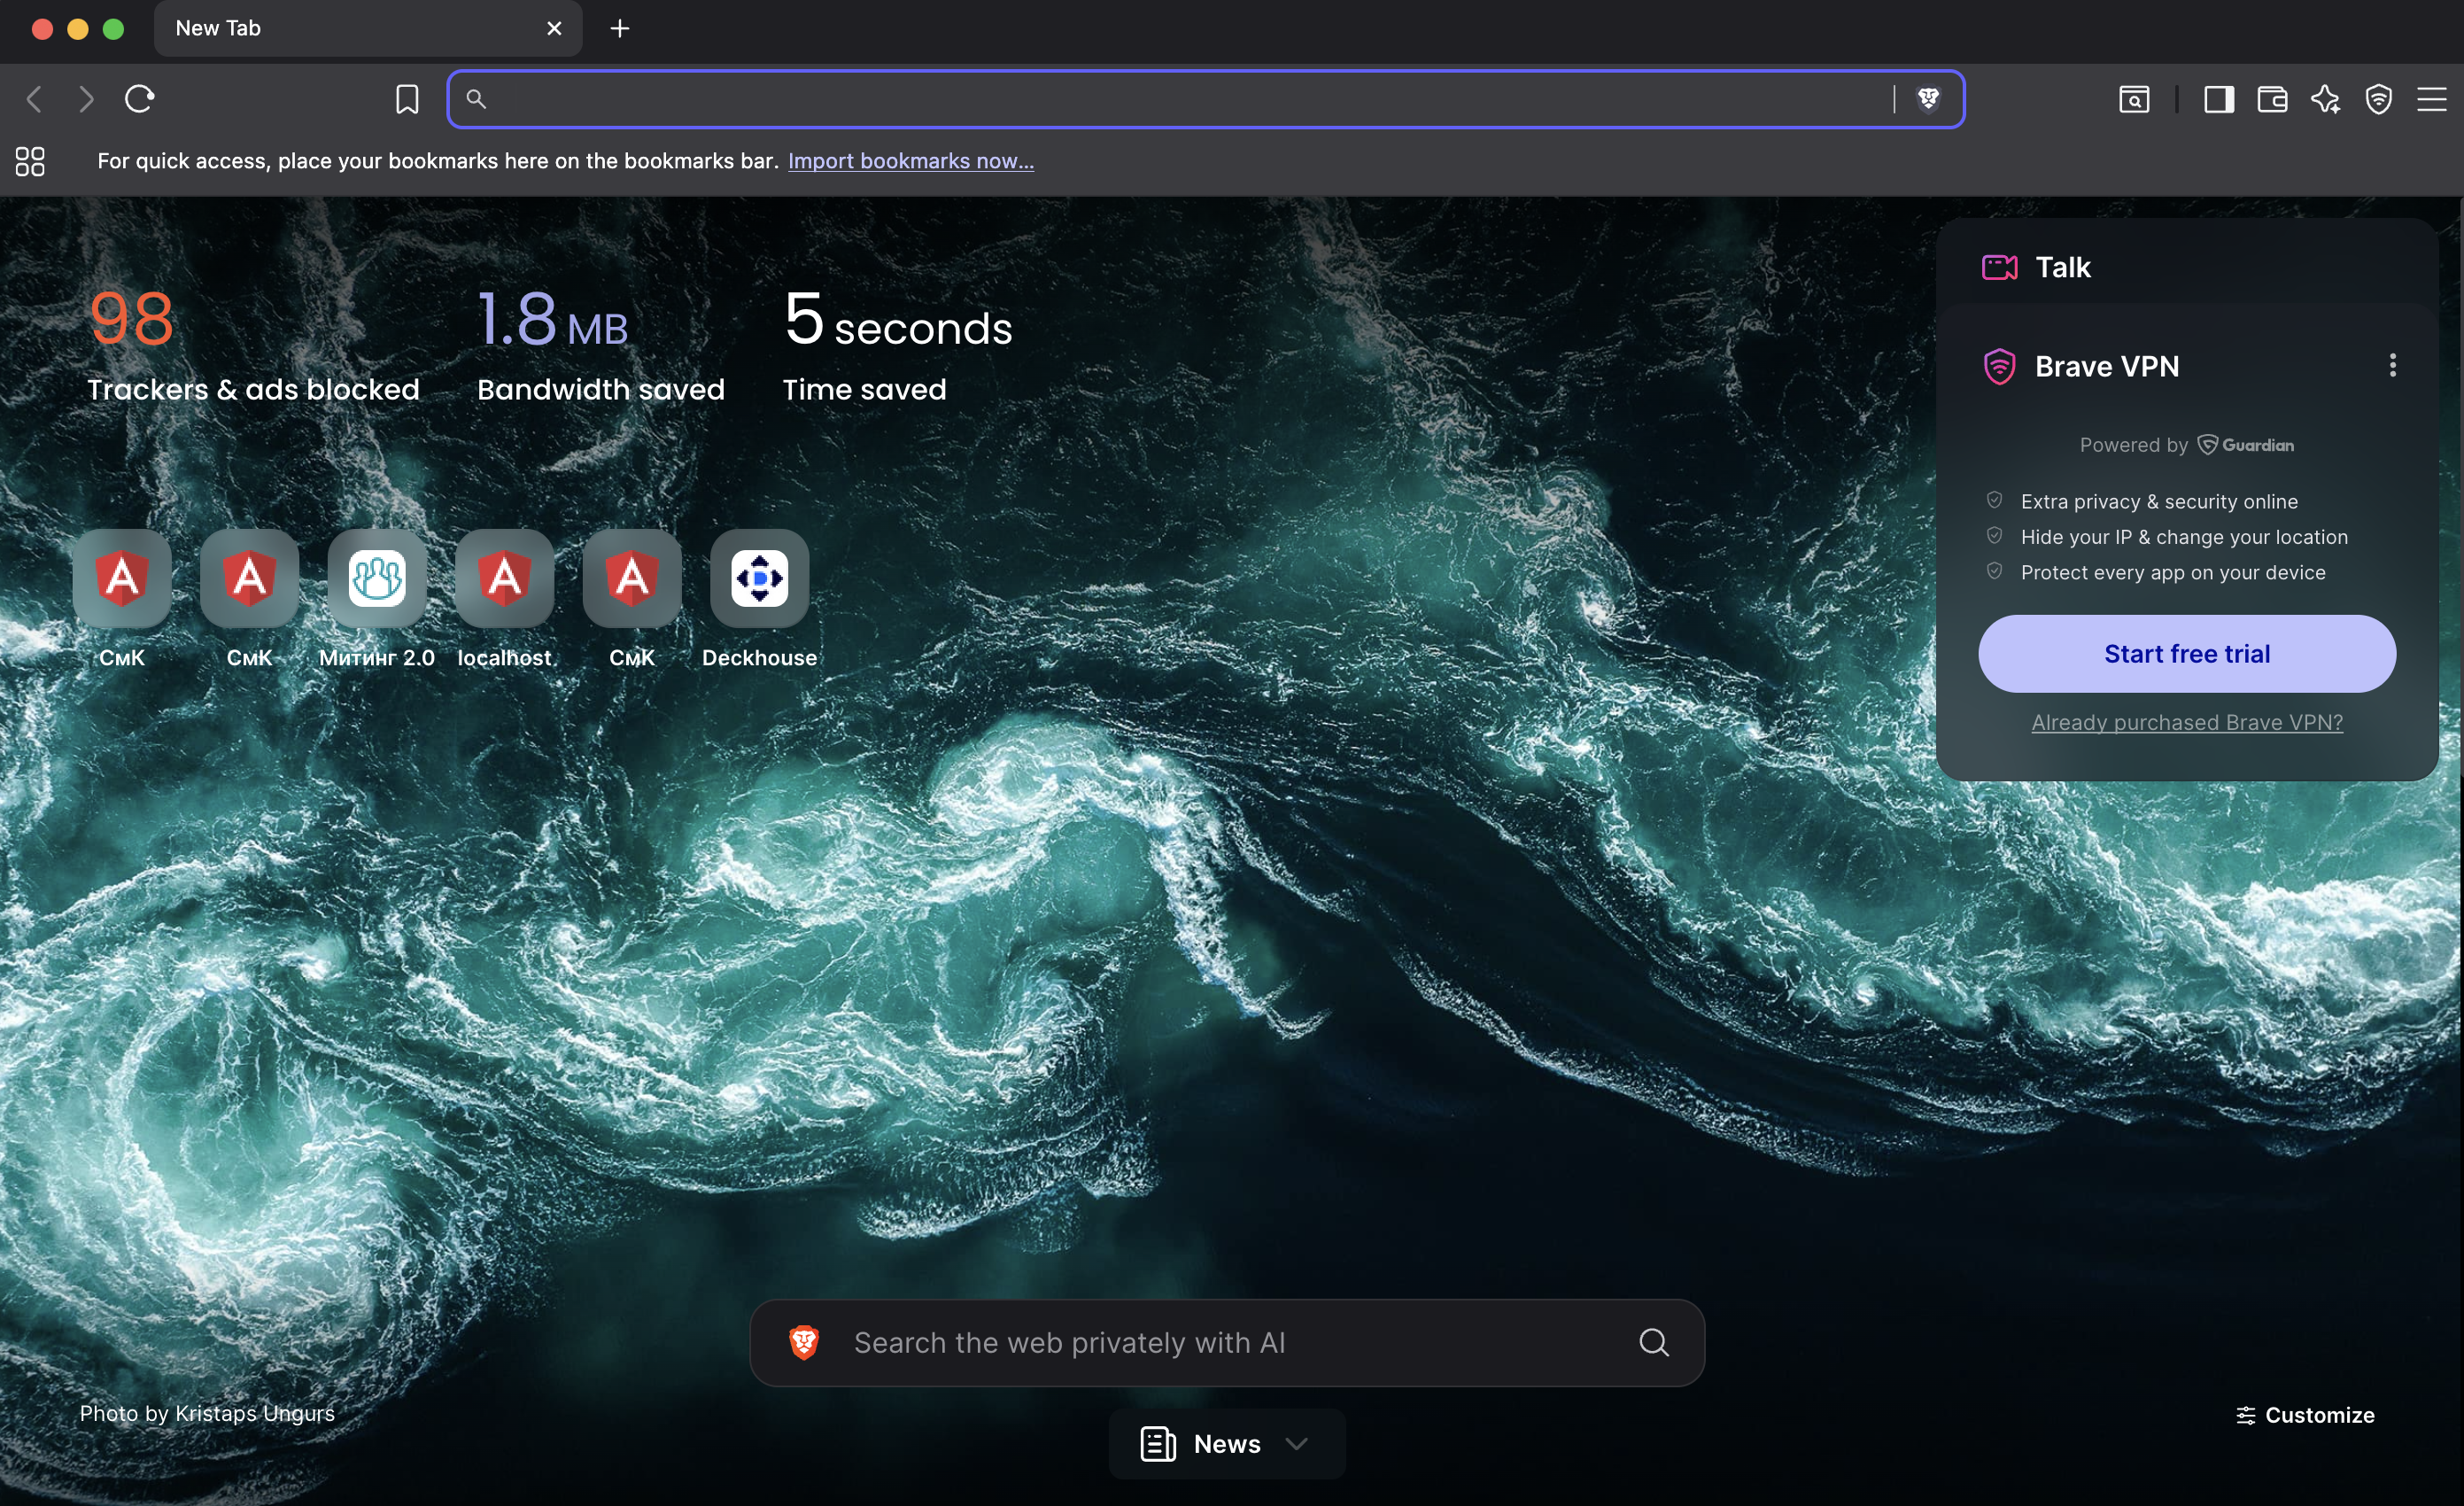
\includegraphics[width=.9\textwidth]{br}
\end{center}

Нашёл в настроках безопасности и конфиденциальности следующие настройки:

\begin{center}
  \includegraphics[width=.9\textwidth]{1}
\end{center}
 
\begin{itemize}
  \item Включил более агрессивную блокировку трекеров и рекламы.
  \item Включил более строгое преобразование подключений в https.
  \item Включил стирание куков после закрытия сайта (и других данных).
\end{itemize}

Почистил куки и данные с сайтов.
\begin{center}
  \includegraphics[width=.9\textwidth]{pas}
\end{center}

Далее выставил настройку, чтобы браузер стирал автоматически все данные при закрытии.

\begin{center}
  \includegraphics[width=.9\textwidth]{2}
\end{center}

Включил стандартную защиту от сомнительных сайтов (при скачивании файлов, просмотре сайтов) и расширений.

\begin{center}
  \includegraphics[width=.9\textwidth]{3}
\end{center}

Сделал все permission чтобы браузер спрашивал доступ к устройству.

\begin{center}
  \includegraphics[width=.9\textwidth]{4}
\end{center}

В браузере есть проверка моей защищённости от взлома.

\begin{center}
  \includegraphics[width=.9\textwidth]{5}
\end{center}

\section{Анализ трафика}

Открытая консоль разработчика

\begin{center}
  \includegraphics[width=.9\textwidth]{6}
\end{center}

Перешёл на сайт VSC.

\begin{center}
  \includegraphics[width=.9\textwidth]{7}
\end{center}

Нашёл один из GET запросов.

\begin{center}
  \includegraphics[width=.9\textwidth]{8}
\end{center}

Запрос был выполнен методом GET, данных в теле запроса не передавалось.

В ответе много стандартных технических заголовков для безопасности (nosniff), идентификации (X-Request-Id, X-Tracking-Ref), сжатия (gzip) и управления кешированием (no-store, no-cache).

Присутствуют параметры CORS (Access-Control-Allow-Origin: *), что разрешает междоменные запросы на этот ресурс.

\begin{center}
  \includegraphics[width=.9\textwidth]{9}
\end{center}
В данном GET-запросе передаётся стандартный набор заголовков, определяющих:
\begin{itemize}
  \item Accept: Клиент ожидает различные типы контента, включая HTML, XML, изображения в форматах avif, webp, apng.
  \item Accept-Encoding: gzip, deflate, br, zstd — поддерживаемые алгоритмы сжатия данных для ответа.
  \item Accept-Language: en-US, en — основной язык общения клиента с сервером (английский).
  \item Cache-Control: max-age=0 — запрещает кэширование ответа, требует свежий контент.
  \item Connection: keep-alive — соединение остаётся открытым для возможных дальнейших запросов.
  \item Host: vcs.gazpromcps.ru — имя целевого сервера.
  \item Sec-CH-UA, Sec-CH-UA-Mobile, Sec-CH-UA-Platform: Информация о бренде браузера (Chromium, Brave), мобильности (?1), платформе ("Android").
  \item Sec-Fetch-Dest, Mode, Site, User: Контекст запроса (document, navigate, cross-site, пользователя).
  \item Sec-GPC: 1 — indicates user opted for privacy (Global Privacy Control).
  \item Upgrade-Insecure-Requests: 1 — клиент запрашивает обновление с http на https при возможности.
  \item User-Agent: Mozilla/5.0 (Linux; Android 6.0; Nexus 5 ... Chrome/140.0.0.0 Mobile) — подробные сведения о платформе, системе, браузере, его версии
\end{itemize}

\begin{center}
  \includegraphics[width=.9\textwidth]{10}
\end{center}

\begin{itemize}
  \item Access-Control-Allow-Origin: * (разрешён кросс-доменный доступ)
  \item Cache-Control: no-store (кэширование запрещено)
  \item Connection: keep-alive (удержание соединения)
  \item Content-Length: 53 (размер JSON-ответа в байтах)
  \item Content-Security-Policy: frame-ancestors 'self' (ответ может быть открыт во фрейме только на своём же источнике)
  \item Content-Type: application/json (ответ в формате JSON)
  \item Date: Wed, 24 Sep 2025 18:06:43 GMT
  \item Keep-Alive: timeout=3, max=5; timeout=5, max=100
  \item Pragma: no-cache (отключение кэширования)
  \item Referrer-Policy: strict-origin-when-cross-origin
  \item Server: Apache
  \item Vary: Origin (зависимость кеширования от варианта Origin)
  \item X-Content-Type-Options: nosniff (браузеру запрещено определять MIME-тип “на лету”, повышает безопасность)
  \item X-Execution-Time: 45212 (время обработки на сервере, мс)
  \item X-Frame-Options: sameorigin (ответ может быть открыт во фрейме только на том же источнике)
\end{itemize}

\begin{center}
  \includegraphics[width=.9\textwidth]{11}
\end{center}

\begin{itemize}
  \item Accept: application/json, text/plain, */* --- ожидаемые форматы ответа
  \item Accept-Encoding: gzip, deflate, br, zstd --- поддерживаемые способы сжатия данных
  \item Accept-Language: en-US, en;q=0.9 --- предпочтительные языки ответа
  \item Connection: keep-alive --- поддержание постоянного соединения
  \item Host: vcs.gazpromcps.ru --- целевой сервер запроса
  \item Referer: https://vcs.gazpromcps.ru/c/7809403647/conference --- адрес отправителя запроса
  \item Sec-Ch-Ua: "Chromium";v="140", "Not-A?Brand";v="24", "Brave";v="140" --- информация о браузере
  \item Sec-Ch-Ua-Mobile: ?1 --- признак мобильного устройства
  \item Sec-Ch-Ua-Platform: "Android" --- платформа устройства
  \item Sec-Fetch-Dest: empty --- цель запроса (API, не страница)
  \item Sec-Fetch-Mode: cors --- использование CORS политики
  \item Sec-Fetch-Site: same-origin --- запрос с того же источника
  \item Sec-Gpc: 1 --- глобальная настройка приватности
  \item User-Agent: Mozilla/5.0 (Linux; Android 6.0; Nexus 5 Build/MRA58N) AppleWebKit/537.36 (KHTML, like Gecko) Chrome/140.0.0.0 Mobile Safari/537.36 --- информация о браузере и устройстве
\end{itemize}

\section{Форма входа}

\begin{center}
  \includegraphics[width=.9\textwidth]{12}
\end{center}

Попробуем отправить admin admin 
\begin{center}
  \includegraphics[width=.9\textwidth]{13}
\end{center}
Данные логина и пароля в данном случае передаются в открытом виде (без явного шифрования на клиенте) в теле POST-запроса. За их безопасность отвечает только защищённое HTTPS-соединение между клиентом и сервером. Если бы трафик передавался по HTTP, пароль и логин были бы уязвимы для перехвата. Дополнительного шифрования или маскирования на уровне данных формы не наблюдается.

\section*{Результаты}
Изучил настройки безопасности браузера и понял, какие данные передаются между
браузером и сайтом.

\end{document}

\begin{center}
  \includegraphics[width=.9\textwidth]{posts}
\end{center}

\href{https://github.com/Alex-de-bug/security-lab-1/actions/runs/17864752066}{Последний верный CI} (https://github.com/Alex-de-bug/security-lab-1/actions/runs/17864752066)

\begin{lstlisting}
  </div><script>alert(1);</script><div>
\end{lstlisting}